\chapter{Marco teórico} \label{chap:background}

En este capítulo se presentan los fundamentos teóricos que sustentan el desarrollo de la metodología en este trabajo. Se abordan cuatro frentes: los sistemas de recomendación junto con sus métricas de evaluación (Sección~\ref{sec:recsys}); la optimización multiobjetivo y la eficiencia de Pareto, marco en el que se formaliza el \textit{trade-off} relevancia--cobertura que persigue este trabajo (Sección~\ref{sec:moo}); los fundamentos de procesamiento de lenguaje natural sobre los que se construye la extracción de aspectos y sentimientos a partir de las reseñas (Sección~\ref{sec:nlp}); y los modelos de recomendación que incorporan la información extraída por ABSA como señal explícita (Sección~\ref{sec:absa_rs}).

%% ============================================================
%% 2.1  SISTEMAS DE RECOMENDACIÓN
%% ============================================================
\section{Sistemas de recomendación} \label{sec:recsys}

Un sistema de recomendación (SR) es un sistema de filtrado de información diseñado para predecir una puntuación que refleje la experiencia real de un usuario con respecto a un ítem con el cual no ha interactuado previamente. Formalmente, el problema se define como la estimación de una función de utilidad:
\begin{equation} \label{eq:utility}
	\hat{r}_{u,i} = f(u, i; \Theta)
\end{equation}
donde $f : \mathcal{U} \times \mathcal{I} \rightarrow \mathbb{R}$ es un escalar, $u \in \mathcal{U}$ representa un usuario, $i \in \mathcal{I}$ un ítem, $\Theta$ los parámetros del modelo y $\hat{r}_{u,i} \in \mathbb{R}$ es la puntuación que el SR asigna al item $i$ para el usuario $u$. De forma general, el conjunto de interacciones observadas $\mathcal{O} = \{(u,i) \mid a_{u,i} \neq 0\}$ se organiza en una \textit{matriz de interacciones} $\mathbf{A} \in \mathbb{R}^{|\mathcal{U}|\times|\mathcal{I}|}$, donde $a_{u,i}$ denota la interacción entre el usuario $u$ y el item $i$, y las mayoría de las entradas permanecen desconocidas \citep{adomavicius_toward_2005}.

Además, la interacción $a_{u,i}$ entre un usuario y un ítem puede ser definida de distintas formas, siendo la más común como una \textit{calificación asignada}. La escala de la calificación varía conforme a los sistemas, la mayoría utilizan la escala 1-5 estrellas, mientras que otros pueden utilizar escalas binarias (interesado/no interesado). La interacción también puede ser definida como una \textit{retroalimentación implícita}, haciendo referencia a variables de acción por parte del usuario con respecto a un ítem \citep{oard1998implicit}. En este caso, las escalas de las interacciones pueden ser muy diversas, prácticamente, podría ser cualquier interacción usuario - ítem que funcione como señal del gusto o disgusto del usuario (e.g. tiempo de lectura en un libro, número de reproducciones de una canción, etc.).

El problema de inferencia en los SR consiste en estimar $\hat{r}_{u,i}$ para todo par $(u,i) \notin \mathcal{O}$. A partir de estas predicciones, las recomendaciones para el usuario $u$ se obtienen seleccionando los $K$ ítems no visitados con mayor puntuación estimada:
\begin{equation} \label{eq:topk}
	\text{Top-}K(u) = \underset{i \in \mathcal{I} \setminus \mathcal{I}_u}{\operatorname{arg\,top\text{-}}K}\; \hat{r}_{u,i}
\end{equation}
donde $\mathcal{I}_u = \{i \in \mathcal{I} \mid a_{u,i} \neq 0\}$ es el conjunto de ítems con los que el usuario $u$ ya ha interactuado.

Los SR se clasifican tradicionalmente en tres familias: filtrado colaborativo, filtrado basado en contenido y sistemas híbridos \citep{sarkar_tourism_2023}. La diferencia entre los enfoques radica en cómo se parametriza $f$ y qué información se utiliza para estimar $\Theta$. A continuación se formalizan cada una de estas aproximaciones.

% --------------------------------------------------------------
\subsection{Filtrado colaborativo} \label{subsec:cf}

El filtrado colaborativo (FC) se fundamenta en la hipótesis de que usuarios con comportamientos similares en el pasado tendrán preferencias similares en el futuro. El FC no requiere información sobre las características de los ítems; opera exclusivamente sobre la matriz de calificaciones $R \in \mathbb{R}^{|\mathcal{U}|\times|\mathcal{I}|}$. Los métodos de FC se dividen en dos categorías: basados en memoria y basados en modelo.

\subsubsection{Basado en memoria} \label{subsubsec:cf_memory}

Los métodos basados en memoria generan predicciones directamente a partir de las interacciones históricas, sin aprender un modelo paramétrico explícito ($\Theta = \emptyset$). Se distinguen dos variantes: basado en usuarios y basado en ítems.

\begin{itemize}
	\item \textbf{FC basado en usuarios.}
	      La predicción para un usuario $u$ sobre un ítem $i$ se calcula como el promedio ponderado de las calificaciones de los usuarios más similares a $u$ que han calificado el ítem $i$:
	      \begin{equation} \label{eq:user_cf}
		      \hat{r}_{u,i} = \bar{r}_u + \frac{\displaystyle\sum_{v \in \mathcal{N}_k(u)} \mathrm{sim}(u, v) \cdot (r_{v,i} - \bar{r}_v)}{\displaystyle\sum_{v \in \mathcal{N}_k(u)} |\mathrm{sim}(u, v)|}
	      \end{equation}
	      donde $\bar{r}_u$ es la calificación promedio del usuario $u$, $\mathcal{N}_k(u)$ denota los $k$ vecinos más similares a $u$ que han calificado el ítem $i$, y $\mathrm{sim}(u, v)$ es una medida de similitud entre usuarios. Las medidas más utilizadas son la similitud coseno (Eq. \ref{eq:cosine}) y la correlación de Pearson (Eq. \ref{eq:pearson}):
	      \begin{equation} \label{eq:cosine}
		      \mathrm{sim}_{\cos}(u, v) = \frac{\displaystyle\sum_{i \in \mathcal{I}_{u,v}} r_{u,i} \cdot r_{v,i}}{\sqrt{\displaystyle\sum_{i \in \mathcal{I}_{u,v}} r_{u,i}^2} \cdot \sqrt{\displaystyle\sum_{i \in \mathcal{I}_{u,v}} r_{v,i}^2}}
	      \end{equation}

	      \begin{equation} \label{eq:pearson}
		      \mathrm{sim}_{\mathrm{Pearson}}(u, v) = \frac{\displaystyle\sum_{i \in \mathcal{I}_{u,v}} (r_{u,i} - \bar{r}_u)(r_{v,i} - \bar{r}_v)}{\sqrt{\displaystyle\sum_{i \in \mathcal{I}_{u,v}} (r_{u,i} - \bar{r}_u)^2} \cdot \sqrt{\displaystyle\sum_{i \in \mathcal{I}_{u,v}} (r_{v,i} - \bar{r}_v)^2}}
	      \end{equation}
	      donde $\mathcal{I}_{uv} = \{i \in \mathcal{I} \mid r_{ui} \neq 0 \land r_{vi} \neq 0\}$ es el conjunto de ítems co-calificados por ambos usuarios.

	\item \textbf{FC basado en ítems.}
	      De manera análoga, la similitud se calcula entre ítems en lugar de entre usuarios. La predicción se obtiene como:
	      \begin{equation} \label{eq:item_cf}
		      \hat{r}_{ui} = \frac{\displaystyle\sum_{j \in \mathcal{N}_k(i)} \mathrm{sim}(i, j) \cdot r_{uj}}{\displaystyle\sum_{j \in \mathcal{N}_k(i)} |\mathrm{sim}(i, j)|}
	      \end{equation}
	      donde $\mathcal{N}_k(i)$ son los $k$ ítems más similares a $i$ que el usuario $u$ ha calificado. Este enfoque tiende a ser más escalable que el basado en usuarios cuando $|\mathcal{U}| \gg |\mathcal{I}|$, ya que las similitudes entre ítems son más estables en el tiempo.

\end{itemize}

Ambas variantes enfrentan limitaciones inherentes: la complejidad computacional para el cálculo de similitudes es $O(|\mathcal{U}|^2 \cdot |\mathcal{I}|)$ u $O(|\mathcal{I}|^2 \cdot |\mathcal{U}|)$, su rendimiento se degrada en matrices con alta dispersión, y no pueden generar recomendaciones para usuarios o ítems nuevos (este problema es conocido como \textit{cold-start}, se abordará en la sección \ref{subsec:cold_start}).

\subsubsection{Basado en modelo} \label{subsubsec:cf_model}

Los métodos basados en modelo aprenden una representación paramétrica compacta de los patrones de interacción. La técnica más establecida es la \textbf{factorización matricial} (FM), que descompone la matriz de utilidad en el producto de dos matrices de menor dimensionalidad \citep{koren_matrix_2009}:
\begin{equation} \label{eq:mf}
	\mathbf{R} \approx \mathbf{P} \mathbf{Q}^\top
\end{equation}
donde $\mathbf{P} \in \mathbb{R}^{|\mathcal{U}| \times k}$ y $\mathbf{Q} \in \mathbb{R}^{|\mathcal{I}| \times k}$ representan las matrices de factores latentes de usuarios e ítems, respectivamente, y $k \ll \min(|\mathcal{U}|, |\mathcal{I}|)$ es la dimensionalidad del espacio latente. Cada fila $\mathbf{p}_u \in \mathbb{R}^k$ codifica las preferencias del usuario $u$, y cada fila $\mathbf{q}_i \in \mathbb{R}^k$ las características latentes del ítem $i$, de modo que la predicción se obtiene como:
\begin{equation} \label{eq:mf_pred}
	\hat{r}_{ui} = \mathbf{p}_u^\top \mathbf{q}_i
\end{equation}

Para estimar los parámetros, se minimiza el error cuadrático regularizado sobre las interacciones observadas $\mathcal{K}$:
\begin{equation} \label{eq:mf_loss}
	\min_{\mathbf{P}, \mathbf{Q}} \sum_{(u,i) \in \mathcal{K}} \left( r_{ui} - \mathbf{p}_u^\top \mathbf{q}_i \right)^2 + \lambda \left( \|\mathbf{p}_u\|^2 + \|\mathbf{q}_i\|^2 \right)
\end{equation}
donde $\lambda > 0$ es el coeficiente de regularización que previene el sobreajuste. Esta optimización se resuelve típicamente mediante descenso por gradiente estocástico (SGD) o mínimos cuadrados alternados (ALS).

Se consideran las siguientes variantes relevantes para este trabajo:
\begin{itemize}
	\item \textbf{SVD} (\textit{Singular Value Decomposition}): Extiende la Ecuación~(\ref{eq:mf_pred}) incorporando sesgos de usuario e ítem:
	      \begin{equation} \label{eq:svd_bias}
		      \hat{r}_{ui} = \mu + b_u + b_i + \mathbf{p}_u^\top \mathbf{q}_i
	      \end{equation}
	      donde $\mu$ es la media global de calificaciones, $b_u$ el sesgo del usuario y $b_i$ el sesgo del ítem.

	\item \textbf{SVD++}: Incorpora retroalimentación implícita al modelo SVD, enriqueciendo la representación del usuario con información de los ítems que ha calificado \citep{koren_factorization_2008}:
	      \begin{equation} \label{eq:svdpp}
		      \hat{r}_{ui} = \mu + b_u + b_i + \left( \mathbf{p}_u + |\mathcal{I}_u|^{-\frac{1}{2}} \sum_{j \in \mathcal{I}_u} \mathbf{y}_j \right)^\top \mathbf{q}_i
	      \end{equation}
	      donde $\mathcal{I}_u$ es el conjunto de ítems calificados por $u$ y $\mathbf{y}_j \in \mathbb{R}^k$ son vectores que capturan la influencia implícita de haber interactuado con el ítem $j$.

	\item \textbf{NMF} (\textit{Non-negative Matrix Factorization}): Impone la restricción $\mathbf{P} \geq 0$, $\mathbf{Q} \geq 0$, lo que produce representaciones aditivas más interpretables, donde cada factor latente contribuye exclusivamente de forma positiva a la predicción.
\end{itemize}

% --------------------------------------------------------------
\subsection{Filtrado basado en contenido} \label{subsec:cbf}

El filtrado basado en contenido (FBC) recomienda ítems cuyas características son similares a las de ítems previamente preferidos por el usuario \citep{pazzani_content_2007}. A diferencia del FC, el FBC opera sobre una descripción explícita de los atributos de los ítems y no requiere información de otros usuarios. Arquitectónicamente, un sistema de FBC se compone de tres módulos \citep{lops_content-based_2011}: (1) un \textit{analizador de contenido} que extrae características de los ítems a partir de su descripción, (2) un \textit{aprendiz de perfil} que construye y actualiza el modelo de preferencias del usuario a partir de su historial de interacciones, y (3) un \textit{componente de filtrado} que genera recomendaciones comparando el perfil del usuario con las representaciones de los ítems candidatos.

\subsubsection*{Representación de ítems}

Cuando los ítems se describen mediante texto no estructurado (reseñas, artículos, descripciones de productos), la representación más empleada es el \textbf{Modelo de Espacio Vectorial} (VSM) con ponderación TF-IDF \citep{lops_content-based_2011, aggarwal_recommender_2016}. Dado un corpus de $N$ documentos y un diccionario $T = \{t_1, \ldots, t_n\}$, el peso del término $t_k$ en el documento $d_j$ se define como:
\begin{equation} \label{eq:tfidf}
	\text{TF-IDF}(t_k, d_j) = \frac{f_{k,j}}{\max_z f_{z,j}} \cdot \log \frac{N}{n_k}
\end{equation}
donde $f_{k,j}$ es la frecuencia de $t_k$ en $d_j$, $\max_z f_{z,j}$ normaliza por el término más frecuente del documento, y $n_k$ es el número de documentos en los que $t_k$ aparece al menos una vez. El ítem $i$ queda representado como el vector normalizado $\boldsymbol{\phi}(i) \in \mathbb{R}^{|T|}$ de sus pesos TF-IDF. Cuando los ítems poseen atributos estructurados (e.g.\ género cinematográfico, valoración numérica por categoría, sentimiento promedio por aspecto derivado de reseñas), el perfil del ítem se construye directamente como un vector $\boldsymbol{\phi}(i) \in \mathbb{R}^d$ de $d$ características, produciendo representaciones más compactas e interpretables \citep{zhang_explicit_2014}.

\subsubsection*{Perfil del usuario y predicción}

El perfil del usuario $\boldsymbol{\theta}(u) \in \mathbb{R}^d$ se construye como el promedio ponderado por calificación de los perfiles de ítems con los que ha interactuado:
\begin{equation} \label{eq:user_profile_cbf}
	\boldsymbol{\theta}(u) = \frac{\displaystyle\sum_{i \in \mathcal{I}_u} r_{u,i} \cdot \boldsymbol{\phi}(i)}{\displaystyle\sum_{i \in \mathcal{I}_u} r_{u,i}}
\end{equation}
donde $r_{u,i}$ es la calificación del usuario $u$ sobre el ítem $i$ e $\mathcal{I}_u$ el conjunto de ítems con los que el usuario ha interactuado. La predicción para un par $(u, i) \notin \mathcal{O}$ se obtiene entonces mediante la similitud coseno entre ambos perfiles:
\begin{equation} \label{eq:cbf}
	\hat{r}_{u,i} = \mathrm{sim}\!\left(\boldsymbol{\theta}(u), \boldsymbol{\phi}(i)\right) = \frac{\boldsymbol{\theta}(u)^\top \boldsymbol{\phi}(i)}{\|\boldsymbol{\theta}(u)\| \cdot \|\boldsymbol{\phi}(i)\|}
\end{equation}

\subsubsection*{Ventajas y limitaciones}

El FBC presenta ventajas estructurales sobre el FC:
\begin{itemize}
	\item \textbf{Independencia del usuario.} Las recomendaciones se generan a partir del perfil del usuario activo sin depender de las interacciones de terceros, eliminando el problema de vecindad escasa.
	\item \textbf{Transparencia.} Las recomendaciones pueden justificarse enumerando las características del ítem que coinciden con el perfil del usuario, a diferencia del FC que opera como caja negra.
	\item \textbf{Cold-start de ítems.} Un ítem nuevo puede recomendarse en cuanto se disponga de su representación de características, sin requerir calificaciones previas de otros usuarios.
\end{itemize}

No obstante, el FBC presenta limitaciones inherentes:
\begin{itemize}
	\item \textbf{Sobre-especialización.} El sistema recomienda ítems similares a los ya preferidos, reduciendo la diversidad y dificultando la aparición de recomendaciones sorpresivas (\textit{serendipity}).
	\item \textbf{Análisis de contenido limitado.} La calidad de las recomendaciones está acotada por la riqueza de la representación de características; atributos latentes o cualidades subjetivas no capturadas por los descriptores quedan fuera del alcance del modelo \citep{aggarwal_recommender_2016}.
	\item \textbf{Cold-start de usuario.} Se requiere un número mínimo de interacciones para construir un perfil informativo; con pocas calificaciones disponibles, las predicciones son poco confiables.
\end{itemize}

% --------------------------------------------------------------
\subsection{Sistemas híbridos} \label{subsec:hybrid}

Los sistemas híbridos combinan múltiples estrategias de recomendación para compensar las debilidades individuales de cada enfoque \citep{raza_comprehensive_2025, sarkar_tourism_2023}. \citep{burke_hybrid_2002} propuso una taxonomía ampliamente adoptada que identifica siete clases de hibridación: \textit{ponderada}, \textit{conmutación}, \textit{mixto}, \textit{combinación de características}, \textit{cascada}, \textit{aumento de características} y \textit{meta-nivel}. La revisión sistemática de \citet{cano_hybrid_2019} sobre 76 publicaciones del periodo 2005--2015 confirma la vigencia de esta taxonomía y reporta que la mayoría de los sistemas combinan FC con otra técnica, siendo la hibridación ponderada la estrategia predominante (28.9\% de los estudios) seguida por la combinación de características (15.8\%).

\begin{description}
	\item[Ponderada.] La puntuación final se obtiene mediante una combinación lineal de las predicciones de cada recomendador individual, asignando pesos que pueden ser globales, por usuario o adaptativos según retroalimentación. \citet{decampos_combining_2010} ejemplifican esta estrategia integrando un módulo de FC y otro de FBC mediante una red bayesiana cuyos parámetros condicionales actúan como factores de ponderación, alcanzando mejoras frente a cada componente individual. La sencillez de su formulación y la facilidad para ajustar la influencia relativa de cada componente explican su popularidad.

	\item[Combinación de características.] Las salidas de un recomendador se incorporan como características adicionales al conjunto de datos sobre el que opera el segundo recomendador (típicamente un FBC, que explota intensivamente atributos del ítem). De esta forma, la información colaborativa se integra como una variable explicativa más, reduciendo la sensibilidad a la dispersión de la matriz original.

	\item[Cascada.] El proceso de recomendación es secuencial: una primera técnica genera un conjunto preliminar de candidatos y una segunda técnica refina dicho conjunto. Es sensible al orden de aplicación de los recomendadores, ya que la segunda etapa solo opera sobre los ítems supervivientes de la primera, lo que la hace eficiente computacionalmente y robusta frente a clasificaciones imprecisas en las primeras posiciones.

	\item[Conmutación.] El sistema alterna dinámicamente entre distintas técnicas de acuerdo con un criterio (e.g., confianza de la predicción, disponibilidad de datos, contexto del usuario). El recomendador de noticias DailyLearner \citep{billsus_learning_2000} ilustra esta clase: emplea un modelo CBF de corto plazo basado en clasificación por vecinos cercanos y, cuando una noticia carece de vecinos cercanos, conmuta a un modelo de largo plazo basado en un clasificador Naive Bayes que captura las preferencias generales del usuario.

	\item[Aumento de características.] Una técnica genera predicciones o clasificaciones que enriquecen las características procesadas por la segunda. A diferencia de \textit{feature combination}, los datos originales del segundo recomendador no se modifican; en su lugar, se le añaden atributos sintéticos. Libra \citep{mooney_content-based_2000} es un recomendador de libros basado en contenido que aumenta las características textuales con los campos ``autores relacionados'' y ``títulos relacionados'' obtenidos del recomendador colaborativo de Amazon, mejorando así la calidad sin modificar el clasificador Naive Bayes subyacente.

	\item[Meta-nivel.] El modelo aprendido por la primera técnica se utiliza íntegramente como entrada de la segunda. La distinción respecto al aumento de características es que aquí no se transfieren atributos individuales, sino una representación compacta del modelo. Fab \citep{balabanovic_fab_1997}, uno de los primeros recomendadores web, construye perfiles vectoriales de usuario con un componente CBF que luego son consumidos por agentes colaborativos para identificar comunidades de intereses afines.

	\item[Mixto.] Las listas de recomendaciones generadas por cada técnica se presentan simultáneamente al usuario, sin ser fusionadas en una única puntuación. Es la forma más simple de hibridación y resulta apropiada cuando se dispone de múltiples recomendadores complementarios. PTV \citep{smyth_personalised_2000}, un sistema de recomendación de programación televisiva, presenta de manera conjunta los resultados de un módulo CBF basado en perfiles de programa y un módulo FC basado en similitud entre usuarios.
\end{description}

En esta tesis se adopta una estrategia de \textbf{combinación ponderada}, donde la predicción final es una combinación lineal convexa de las predicciones de los componentes colaborativo y basado en contenido:
\begin{equation} \label{eq:hybrid}
	\hat{r}_{ui} = \alpha \cdot \hat{r}_{ui}^{\,\mathrm{CF}} + (1 - \alpha) \cdot \hat{r}_{ui}^{\,\mathrm{CBF}}
\end{equation}
donde $\alpha \in [0, 1]$ controla la contribución relativa de cada componente. Esta formulación se extiende naturalmente a un vector de pesos $\boldsymbol{\alpha} = (\alpha_1, \alpha_2, \ldots, \alpha_M)$ cuando se combinan $M$ señales de recomendación, sujeto a $\sum_{m=1}^{M} \alpha_m = 1$.

En esta tesis el híbrido se restringe a la combinación de $M=2$ componentes basados en aspectos, de modo que el vector de pesos puede ser reducido a un único escalar $\alpha \in [0, 1]$. Esta reducción dimensional es determinante: la calibración del peso óptimo no constituye un problema de optimización en un espacio de alta dimensión que demande técnicas metaheurísticas, sino un barrido unidimensional sobre $\alpha$ del que el óptimo se lee directamente. Más aún, la selección de $\alpha$ no responde a un único criterio, sino al compromiso entre relevancia y cobertura, lo que sitúa el problema en el marco de la optimización multiobjetivo desarrollado en la Sección~\ref{sec:moo}.

La integración de señales aspecto-sentimiento en el recomendador, donde los aspectos y sentimientos extraídos por el componente NLP enriquecen tanto los perfiles de usuario como los de ítem, ha demostrado ser efectiva en dominios donde la información textual complementa las calificaciones numéricas. \citet{musto_multi-criteria_2017} mostraron que un FC multi-criterio alimentado con sentimientos por aspecto extraídos automáticamente de reseñas supera tanto a algoritmos de un solo criterio como a técnicas de factorización matricial. Por su parte, \citet{zhang_explicit_2014} propusieron el \textit{Explicit Factor Model} (EFM), que integra factores explícitos derivados de los aspectos y las opiniones de las reseñas con factores latentes en un modelo unificado. Este último enfoque, que sustenta la propuesta de esta tesis, se analiza en detalle en la Sección~\ref{sec:absa_rs}.

% --------------------------------------------------------------
\subsection{Problema del arranque en frío y dispersión} \label{subsec:cold_start}

Dos desafíos fundamentales afectan el rendimiento de los SR, particularmente relevantes en el dominio turístico \citep{sarkar_tourism_2023}: el arranque en frío y la dispersión de la matriz de interacciones. La primera se manifiesta en dos variantes:
\begin{itemize}
	\item \textbf{De usuario}: usuarios nuevos sin historial de calificaciones, para los cuales el FC no puede calcular similitudes. El FBC puede mitigar este problema si se dispone de información demográfica o preferencias explícitas iniciales.
	\item \textbf{De ítem}: ítems nuevos sin calificaciones, invisibles para el FC. En este trabajo, el pipeline de ABSA permite generar un perfil de aspectos para un nuevo Pueblo Mágico a partir de sus reseñas textuales, habilitando recomendaciones basadas en contenido sin historial de calificaciones numéricas.
\end{itemize}

La dispersión del $90.32\%$ en el dataset REST-MEX implica que cada usuario ha calificado, en promedio, menos de $5$ de los $48$ pueblos disponibles. Este nivel de dispersión degrada significativamente el rendimiento de los métodos basados en memoria, ya que la cantidad de ítems co-calificados entre pares de usuarios ($|\mathcal{I}_{uv}|$) tiende a ser pequeña, resultando en estimaciones de similitud poco confiables \citep{raza_comprehensive_2025}. Las principales estrategias de mitigación incluyen: (i)~factorización matricial, que generaliza patrones a partir de factores latentes aun con matrices dispersas; (ii)~incorporación de información lateral (\textit{side information}), como las reseñas textuales; y (iii)~sistemas híbridos que combinan señales complementarias \citep{payandenick_multi-criteria_2025}.

% --------------------------------------------------------------
%

\subsection{Evaluación} \label{subsec:evaluation}

La evaluación de un SR es un problema multifacético cuya configuración requiere decisiones explícitas sobre el tipo de experimento, los datos empleados, el protocolo de partición y el conjunto de métricas reportadas \citep{zangerle_evaluating_2022}. Tradicionalmente se distinguen tres modalidades: \textit{evaluación en línea} (despliegue del sistema sobre usuarios reales y medición de señales como CTR o tasa de conversión), \textit{estudios de usuario} (sujetos reclutados que interactúan con el sistema en un entorno controlado) y \textit{evaluación fuera de línea} (uso de un \textit{snapshot} histórico de interacciones para simular el comportamiento de los usuarios). En la práctica, la evaluación fuera de línea es predominante por su bajo costo, su reproducibilidad y la posibilidad de comparar de forma controlada múltiples configuraciones algorítmicas sobre los mismos datos. Su principal limitación es que mide la capacidad del modelo para reconstruir interacciones ya observadas, no la utilidad percibida por el usuario en un escenario real. La metodología adoptada en este trabajo es de tipo fuera de línea sobre el corpus REST-MEX descrito en el Capítulo~\ref{chap:dataset}.

\subsubsection{Separación de conjuntos de entrenamiento y prueba} \label{subsubsec:train_test_split}

Toda evaluación fuera de línea requiere particionar el conjunto de interacciones $\mathcal{O}$ en un subconjunto de entrenamiento $\mathcal{O}_\text{train}$, sobre el que el SR ajusta sus parámetros, y un subconjunto de prueba $\mathcal{O}_\text{test}$, sobre el que se evalúa la capacidad predictiva. Aunque a primera vista parece una decisión secundaria, \citet{canamares_offline_2020} muestran experimentalmente que la elección del protocolo de partición puede invertir el orden relativo de dos algoritmos comparados sobre el mismo conjunto de datos, lo que convierte a esta etapa en un componente metodológico crítico. Las estrategias más empleadas en la literatura son:
\begin{itemize}
	\item \textbf{División aleatoria.} Cada interacción se asigna a $\mathcal{O}_\text{train}$ o $\mathcal{O}_\text{test}$ con una probabilidad fija (típicamente $80{:}20$ o $50{:}50$), eventualmente bajo un esquema de validación cruzada de $k$ pliegues. Es la opción más simple, pero ignora la dependencia temporal y permite que interacciones futuras de un usuario aparezcan en entrenamiento.
	\item \textbf{Leave-$\ell$-out por usuario.} Para cada usuario con al menos $\ell$ interacciones, se reservan $\ell$ aleatoriamente para prueba. Garantiza que todo usuario participe en la evaluación; el caso $\ell = 1$ se conoce como \textit{leave-one-out}.
	\item \textbf{Asignación por ítem.} Se reserva un número fijo de calificaciones por ítem para entrenamiento, mitigando el sesgo de popularidad que se produce cuando los ítems con muchas calificaciones también tienden a tener muchas en el conjunto de prueba.
	\item \textbf{División temporal.} Las interacciones se ordenan por su \textit{timestamp} y se asignan las más antiguas a $\mathcal{O}_\text{train}$ y las más recientes a $\mathcal{O}_\text{test}$, ya sea con un punto de corte global o por usuario. Esta estrategia es la única que reproduce el escenario realista en el que el SR predice interacciones futuras a partir de información estrictamente pasada, evitando la fuga temporal de información.
\end{itemize}

% Usar esto en metodología.
% En esta tesis se adopta una estrategia \textit{last-month-out} por usuario: para cada $u \in \mathcal{U}$, las reseñas correspondientes al último mes en el que registró actividad se asignan a $\mathcal{O}_\text{test}$ y el resto a $\mathcal{O}_\text{train}$. Esta variante combina las garantías del \textit{leave-$\ell$-out} (todo usuario con suficiente historial es evaluado) con las de la división temporal (no se filtra información futura hacia el modelo), y resulta consistente con la naturaleza estacional de las visitas turísticas a los Pueblos Mágicos.

\subsubsection{Métricas} \label{sec:metrics}

La evaluación de un SR Top-$K$ no se reduce a la fidelidad numérica de la predicción de calificaciones (RMSE, MAE), pues estas métricas no reflejan la calidad del ordenamiento que el usuario realmente percibe. Por ello, las métricas dominantes en la literatura actual operan sobre la lista recomendada y se agrupan en al menos siete familias: precisión predictiva, predicción de uso, \textit{ranking}, novedad, diversidad, cobertura y serendipia. Una configuración de evaluación rigurosa debe reportar simultáneamente varias de estas dimensiones, ya que un SR optimizado para una métrica puede degradar otras sin que ello sea evidente en una evaluación unidimensional.

Sea $\mathcal{R}_u^K = (i_1, \ldots, i_K)$ la lista de los $K$ ítems con mayor puntuación predicha para el usuario $u$ que no pertenecen a $\mathcal{I}_u$, y sea $\text{Rel}(u) \subseteq \mathcal{I}$ el conjunto de ítems considerados relevantes para $u$ en $\mathcal{O}_\text{test}$.

\subsubsection{Métricas de ranking} \label{subsubsec:ranking_metrics}

\paragraph{Precision@K y Recall@K}
La \textit{precisión} a profundidad $K$ es la fracción de ítems recomendados que son relevantes, mientras que la \textit{exhaustividad} (\textit{recall}) mide la fracción de ítems relevantes que el sistema logra recuperar entre los primeros $K$:
\begin{equation} \label{eq:precision_recall}
	\text{P@}K(u) = \frac{|\mathcal{R}_u^K \cap \text{Rel}(u)|}{K}, \qquad \text{R@}K(u) = \frac{|\mathcal{R}_u^K \cap \text{Rel}(u)|}{|\text{Rel}(u)|}.
\end{equation}
Ambas se promedian sobre el conjunto de usuarios. Existe un compromiso natural entre ambas: aumentar $K$ incrementa $\text{R@}K$ a costa de $\text{P@}K$, pues los ítems añadidos al final de la lista tienden a ser menos relevantes.

\paragraph{NDCG@K}
La \textit{Normalized Discounted Cumulative Gain} pondera la posición del ítem en la lista, penalizando los ítems relevantes que aparezcan en posiciones bajas:
\begin{equation} \label{eq:dcg}
	\text{DCG@}K(u) = \sum_{i=1}^{K} \frac{2^{\text{rel}_i} - 1}{\log_2(i+1)}, \qquad \text{NDCG@}K(u) = \frac{\text{DCG@}K(u)}{\text{IDCG@}K(u)},
\end{equation}
donde $\text{rel}_i$ es la relevancia del ítem en la $i$-ésima posición y $\text{IDCG@}K(u)$ es el DCG del ordenamiento ideal sobre los ítems de prueba del usuario, lo que normaliza el valor al intervalo $[0, 1]$. Cuando las calificaciones se emplean como juicios graduados, la transformación $g(r) = 2^{r}-1$ amplifica la contribución de las calificaciones altas frente a las moderadas. NDCG@$K$ es la métrica principal de optimización en esta tesis por dos motivos: (i)~es sensible al orden, lo que se alinea con el carácter de \textit{ranking} de la tarea; y (ii)~es la métrica más reportada en la literatura de SR turísticos, lo que facilita la comparación con trabajos relacionados.

\paragraph{MRR (Mean Reciprocal Rank)}
El \textit{rango recíproco medio} mide qué tan arriba aparece el primer ítem relevante en la lista recomendada:
\begin{equation} \label{eq:mrr}
	\text{MRR} = \frac{1}{|\mathcal{U}|} \sum_{u \in \mathcal{U}} \frac{1}{\text{rank}_u},
\end{equation}
donde $\text{rank}_u$ es la posición del primer ítem de $\text{Rel}(u)$ en $\mathcal{R}_u^K$ (con $1/\text{rank}_u = 0$ si ningún ítem relevante aparece en los primeros $K$). MRR es informativa cuando solo el primer acierto importa, pero ignora el resto de la lista.

\subsubsection{Métricas beyond-accuracy} \label{subsubsec:beyond_accuracy}

\paragraph{Diversidad}
La \textit{intra-list diversity} (ILD) mide la disimilitud promedio entre pares de ítems dentro de una misma lista recomendada:
\begin{equation} \label{eq:ild}
	\text{ILD}(\mathcal{R}_u^K) = \frac{2}{K(K-1)} \sum_{1 \leq i < j \leq K} \bigl(1 - \mathrm{sim}(\boldsymbol{\phi}(i), \boldsymbol{\phi}(j))\bigr),
\end{equation}
donde $\mathrm{sim}(\cdot, \cdot)$ es típicamente la similitud coseno sobre representaciones de ítems. En el contexto turístico, esta métrica es especialmente relevante para evitar recomendar $K$ pueblos pertenecientes al mismo estado o categoría, lo que reduciría el valor experiencial de la recomendación.

\paragraph{Cobertura}
La \textit{cobertura de catálogo} cuantifica la fracción de ítems del sistema que aparecen al menos una vez en alguna recomendación:
\begin{equation} \label{eq:coverage}
	\text{Coverage} = \frac{|\bigcup_{u \in \mathcal{U}} \mathcal{R}_u^K|}{|\mathcal{I}|}.
\end{equation}

Esta métrica es relevante dado el desbalance del dataset REST-MEX, en el que un subconjunto reducido de pueblos concentra la mayoría de las reseñas: un SR podría obtener valores aceptables de NDCG@$K$ recomendando casi exclusivamente esos pueblos populares, sacrificando la exposición del catálogo en su conjunto.

%% ============================================================
%% 2.2  OPTIMIZACIÓN MULTIOBJETIVO Y EFICIENCIA DE PARETO
%% ============================================================
\section{Optimización multiobjetivo y eficiencia de Pareto} \label{sec:moo}

El análisis de las métricas de evaluación reveló que un SR no puede ser juzgado por un único criterio: la relevancia del \textit{ranking} y la cobertura del catálogo son objetivos en conflicto que ningún sistema maximiza simultáneamente. Esta situación es un caso particular de un problema de \textbf{optimización multiobjetivo} (MOO), cuyo marco formal es la \textit{eficiencia de Pareto}. Este marco proporciona las herramientas para razonar sobre soluciones de compromiso. El concepto fue introducido por el economista Vilfredo Pareto en el contexto de la economía del bienestar, donde una asignación de recursos se considera eficiente cuando no es posible mejorar la situación de un agente sin perjudicar la de otro \citep{barr2020economics}, y posteriormente se generalizó como criterio de optimalidad en la teoría de la optimización vectorial \citep{miettinen1999nonlinear}. Esta sección formaliza el problema multiobjetivo, las nociones de dominancia y frente de Pareto, y el método de escalarización que se emplea en este trabajo para resolver el \textit{trade-off} relevancia--cobertura.

% --------------------------------------------------------------
\subsection{Planteamiento del problema multiobjetivo} \label{subsec:moo_problem}

Un problema de optimización multiobjetivo busca optimizar de forma conjunta $k \geq 2$ funciones objetivo sobre un conjunto factible. Adoptando, sin pérdida de generalidad, la convención de minimización (todo objetivo a maximizar $f_i$ se reescribe como $-f_i$), se formula como:
\begin{equation} \label{eq:moo}
	\min_{\mathbf{x} \in \Omega} \; \mathbf{F}(\mathbf{x}) = \bigl(f_1(\mathbf{x}), f_2(\mathbf{x}), \ldots, f_k(\mathbf{x})\bigr),
\end{equation}
donde $\mathbf{x} = (x_1, \ldots, x_n)$ es el \textit{vector de decisión}, $\Omega \subseteq \mathbb{R}^n$ es el \textit{espacio de decisión factible} (definido por las restricciones del problema) y $\mathbf{F}: \Omega \to \mathbb{R}^k$ aplica cada solución a su \textit{vector de objetivos}. La imagen $\mathcal{Z} = \mathbf{F}(\Omega) \subseteq \mathbb{R}^k$ se denomina \textit{región objetivo factible} y es el espacio en el que se evalúan los compromisos entre criterios \citep{miettinen1999nonlinear, deb2011multi}. A diferencia de la optimización escalar ($k=1$), en la que el orden total de $\mathbb{R}$ induce un único óptimo, en $\mathbb{R}^k$ con $k \geq 2$ no existe un orden total natural entre vectores, por lo que el problema (\ref{eq:moo}) carece, en general, de una solución única que minimice todos los objetivos a la vez.

% --------------------------------------------------------------
\subsection{Dominancia y optimalidad de Pareto} \label{subsec:pareto}

El orden parcial que sustituye al orden total escalar es la \textbf{relación de dominancia de Pareto}. Dados dos vectores de objetivos $\mathbf{u}, \mathbf{v} \in \mathbb{R}^k$, se dice que $\mathbf{u}$ \textit{domina} a $\mathbf{v}$ (denotado $\mathbf{u} \prec \mathbf{v}$) si y solo si $\mathbf{u}$ no es peor en ningún objetivo y es estrictamente mejor en al menos uno:
\begin{equation} \label{eq:dominance}
	\mathbf{u} \prec \mathbf{v} \iff \bigl(\forall\, i \in \{1, \ldots, k\}:\; u_i \leq v_i\bigr) \;\wedge\; \bigl(\exists\, i_0 \in \{1, \ldots, k\}:\; u_{i_0} < v_{i_0}\bigr).
\end{equation}
A partir de esta relación, una solución $\mathbf{x}^{\star} \in \Omega$ es \textbf{Pareto-óptima} (o eficiente) si no existe ninguna otra solución factible que la domine en el espacio de objetivos:
\begin{equation} \label{eq:pareto_optimal}
	\mathbf{x}^{\star} \text{ es Pareto-óptima} \iff \nexists\, \mathbf{x} \in \Omega \;:\; \mathbf{F}(\mathbf{x}) \prec \mathbf{F}(\mathbf{x}^{\star}).
\end{equation}
Intuitivamente, en una solución Pareto-óptima no es posible mejorar ningún objetivo sin degradar simultáneamente al menos otro. Se distingue además la \textbf{optimalidad débil de Pareto}, que relaja la condición exigiendo que no exista $\mathbf{x}$ con $f_i(\mathbf{x}) < f_i(\mathbf{x}^{\star})$ para \emph{todos} los objetivos a la vez; toda solución Pareto-óptima es débilmente óptima, pero no a la inversa \citep{miettinen1999nonlinear}.

El conjunto de todas las soluciones Pareto-óptimas en el espacio de decisión se denomina \textbf{conjunto de Pareto}, $\mathcal{P} = \{\mathbf{x}^{\star} \in \Omega : \mathbf{x}^{\star} \text{ es Pareto-óptima}\}$, y su imagen en el espacio de objetivos constituye el \textbf{frente de Pareto}:
\begin{equation} \label{eq:pareto_front}
	\mathcal{PF} = \mathbf{F}(\mathcal{P}) = \{\mathbf{F}(\mathbf{x}^{\star}) : \mathbf{x}^{\star} \in \mathcal{P}\} \subseteq \mathcal{Z}.
\end{equation}
El frente de Pareto es el lugar geométrico de los compromisos eficientes: la frontera de la región factible $\mathcal{Z}$ más allá de la cual no existen soluciones alcanzables. La Figura~\ref{fig:pareto_front} ilustra estos conceptos para un problema biobjetivo. Los puntos $p_1$ y $p_2$ pertenecen al frente (línea gruesa) y son no dominados; en cambio, el punto interior $p_3$ está dominado por $p_1$, que para igual valor de $f_1$ alcanza un menor $f_2$. Resolver un problema multiobjetivo consiste, entonces, en identificar (o aproximar) el frente de Pareto y seleccionar sobre él la solución que mejor refleje las preferencias del decisor.

\begin{figure}
	\centering
	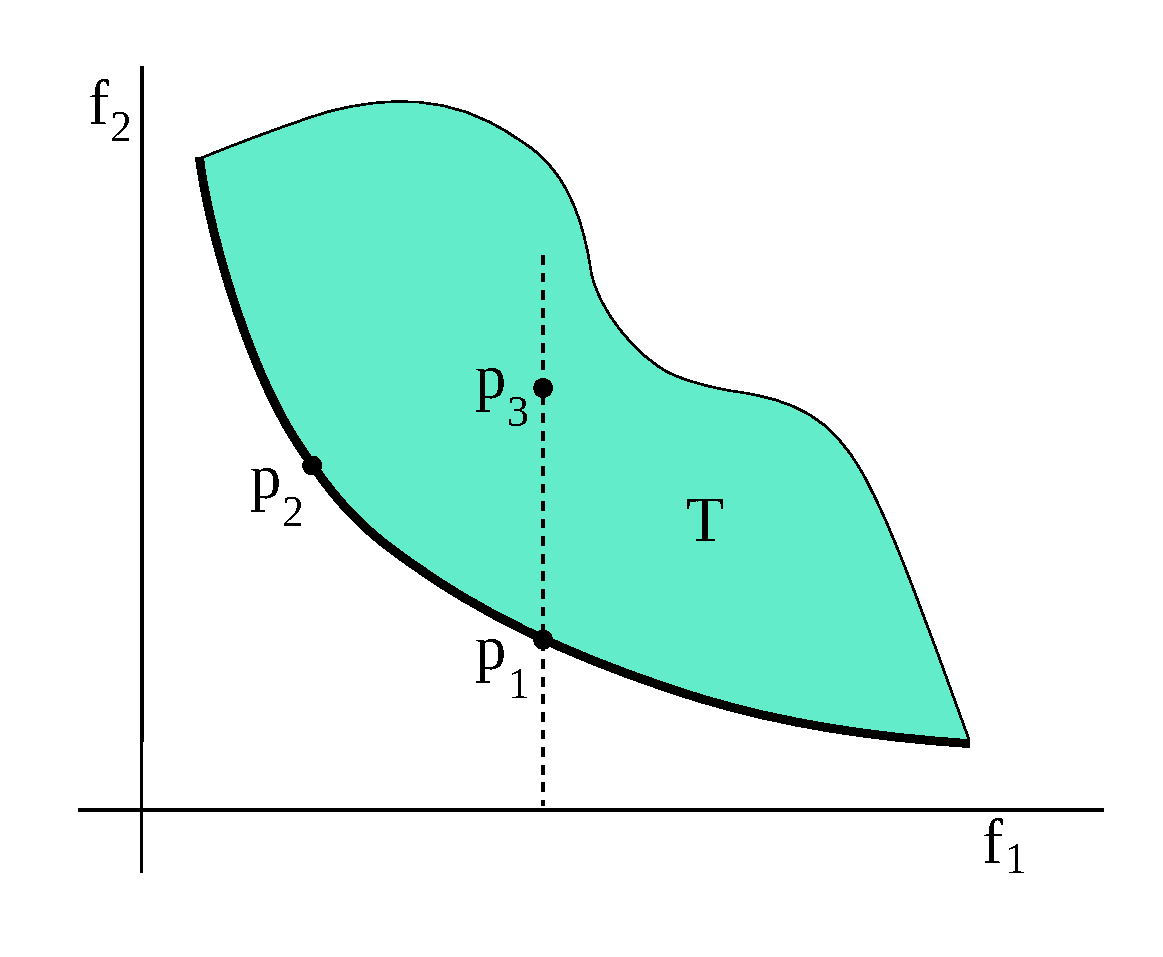
\includegraphics[width=0.6\textwidth]{figures/frente_pareto.pdf}
	\caption[Frente de Pareto de un problema biobjetivo]{Frente de Pareto (línea gruesa) de un problema con dos objetivos a minimizar. El área coloreada $T$ es la imagen de la función objetivo; los puntos $p_1$ y $p_2$ son soluciones no dominadas sobre el frente, mientras que $p_3$ es dominado por $p_1$. En este ejemplo se considera un caso de minimización. Fuente: \href{https://es.wikipedia.org/wiki/Eficiencia_de_Pareto\#/media/Archivo:FrentePareto.svg}{Wikimedia Commons, licencia CC BY-SA 3.0}.}
	\label{fig:pareto_front}
\end{figure}

% --------------------------------------------------------------
\subsection{Escalarización por suma ponderada} \label{subsec:scalarization}

Dado que el frente de Pareto contiene, en general, infinitas soluciones, los métodos de resolución de problemas MOO deben incorporar información de preferencia para seleccionar puntos concretos. Las técnicas \textit{a priori} de \textbf{escalarización} transforman el problema vectorial (\ref{eq:moo}) en una familia de problemas escalares parametrizados, cada uno de los cuales puede resolverse con herramientas de optimización estándar \citep{miettinen1999nonlinear, marler2004survey}. El método de escalarización más difundido es la \textbf{suma ponderada}, que agrega los objetivos en una combinación convexa:
\begin{equation} \label{eq:weighted_sum}
	\min_{\mathbf{x} \in \Omega} \; \sum_{i=1}^{k} w_i\, f_i(\mathbf{x}), \qquad w_i \geq 0, \quad \sum_{i=1}^{k} w_i = 1,
\end{equation}
donde los pesos $w_i$ codifican la importancia relativa asignada a cada objetivo. La propiedad fundamental que justifica el método es que, si todos los pesos son estrictamente positivos ($w_i > 0$), la solución de (\ref{eq:weighted_sum}) es Pareto-óptima; recíprocamente, cuando la región objetivo factible es \textit{convexa}, todo punto del frente de Pareto puede obtenerse para alguna elección de pesos, de modo que barrer el espacio de pesos reconstruye el frente completo \citep{miettinen1999nonlinear}. Esta garantía deja de cumplirse en problemas no convexos: las porciones cóncavas del frente son inalcanzables por la suma ponderada, limitación bien documentada en la literatura \citep{marler2004survey}. Pese a ello, la suma ponderada sigue siendo el método de escalarización de referencia por su transparencia interpretativa y su bajo costo computacional.

% --------------------------------------------------------------
\subsection{Aplicación al trade-off relevancia--cobertura} \label{subsec:tradeoff}

En esta tesis, el problema de seleccionar el peso de fusión del recomendador híbrido se formula como un problema biobjetivo ($k=2$) en el que se busca \emph{maximizar} simultáneamente la relevancia y la cobertura:
\begin{equation} \label{eq:moo_recsys}
	\max_{\alpha \in [0,1]} \; \bigl(\mathrm{NDCG@}K(\alpha),\; \mathrm{Cov@}K(\alpha)\bigr),
\end{equation}
donde el vector de decisión se reduce a un \emph{único escalar} $\alpha$, el peso de la fusión convexa de la Ecuación~(\ref{eq:hybrid}). Aplicando la escalarización por suma ponderada (\ref{eq:weighted_sum}) con un peso de preferencia $\beta \in [0,1]$, el problema vectorial se convierte en la maximización del objetivo escalar:
\begin{equation} \label{eq:scalarization}
	f(\alpha; \beta) = \beta\, \mathrm{NDCG@}K(\alpha) + (1 - \beta)\, \mathrm{Cov@}K(\alpha),
\end{equation}
en el que $\beta = 1$ recupera la optimización pura de relevancia y $\beta = 0$ la de cobertura. Como ambos objetivos se ponderan de forma no negativa, el maximizador de (\ref{eq:scalarization}) es una solución Pareto-óptima del problema (\ref{eq:moo_recsys}).

La particularidad que distingue este planteamiento es que el espacio de decisión es unidimensional. En consecuencia, el óptimo para cada nivel de preferencia,
\begin{equation} \label{eq:alpha_star}
	\alpha^{\star}(\beta) = \arg\max_{\alpha \in [0,1]} \; f(\alpha; \beta),
\end{equation}
se obtiene mediante un \textbf{barrido unidimensional}: se evalúa $f(\alpha; \beta)$ sobre una rejilla de valores de $\alpha$ y se lee el máximo directamente de la curva. Este procedimiento es exacto hasta la resolución de la rejilla y computacionalmente trivial, por lo que \emph{no se requiere recurrir a metaheurísticas} (algoritmos genéticos, enjambre de partículas, evolución diferencial u optimización bayesiana), reservadas para espacios de búsqueda de alta dimensión, multimodales o no diferenciables donde la enumeración exhaustiva es inviable. Finalmente, la trayectoria $\alpha^{\star}(\beta)$ obtenida al variar $\beta \in [0,1]$ recorre el frente de Pareto del sistema y constituye el resultado central del \textit{trade-off} relevancia--cobertura que da título a este trabajo.

%% ============================================================
%% 2.3  PROCESAMIENTO DE LENGUAJE NATURAL
%% ============================================================
\section{Procesamiento de Lenguaje Natural} \label{sec:nlp}

El texto de las reseñas constituye una fuente de información semántica complementaria a las calificaciones numéricas, y suele contener juicios diferenciados sobre múltiples atributos del ítem que la puntuación global agrega en un único escalar. El procesamiento de lenguaje natural (NLP) provee la infraestructura para extraer dicha estructura: codifica el texto en representaciones manipulables algorítmicamente y, sobre ellas, formula tareas de clasificación, etiquetado o generación. Esta sección presenta los fundamentos sobre los que se apoyan los componentes textuales del recomendador propuesto. Se introducen primero las representaciones distribuidas y contextuales sobre las que opera el NLP moderno (Sección~\ref{subsec:text_repr}); a continuación se formaliza el análisis de sentimientos basado en aspectos (ABSA) y sus subtareas (Sección~\ref{subsec:absa_def}); y por último se describen los dos paradigmas instrumentales empleados en este trabajo: la clasificación zero-shot vía inferencia textual para detectar categorías de aspecto (Sección~\ref{subsec:zero_shot}) y la clasificación supervisada con codificadores Transformer ajustados al dominio para inferir polaridad (Sección~\ref{subsec:sentiment_models}).

% --------------------------------------------------------------
\subsection{Representación de texto} \label{subsec:text_repr}

Las primeras representaciones empleadas en NLP discretizaban el texto mediante esquemas de \textit{bag-of-words} y ponderación TF-IDF (Eq.~\ref{eq:tfidf}), produciendo vectores de muy alta dimensionalidad y dispersos que descartaban el orden de las palabras y la ambigüedad semántica \citep{aggarwal_recommender_2016}. Los \textit{word embeddings} densos (e.g. Word2Vec \citep{mikolov_efficient_2013}, GloVe \citep{pennington2014glove}) introdujeron representaciones de baja dimensionalidad $\mathbf{e}_w \in \mathbb{R}^d$ ($d \approx 50$--$300$) entrenadas para preservar relaciones distribucionales entre palabras: vocablos que aparecen en contextos similares quedan cercanos en el espacio vectorial. No obstante, son \textit{embeddings} estáticos: una palabra ambigua como ``banco'' recibe un único vector independientemente de si la oración refiere a una entidad financiera o a un asiento. Los modelos contextuales basados en Transformer \citep{vaswani_attention_2017} subsanan esta limitación produciendo $\mathbf{e}_{w,t} \in \mathbb{R}^d$ \emph{condicionado} al contexto $t$ en el que aparece la palabra \citep{devlin_bert_2019}.

La arquitectura Transformer modela las dependencias entre tokens mediante un mecanismo de \textit{self-attention} escalado:
\begin{equation} \label{eq:attention}
	\mathrm{Attention}(\mathbf{Q}, \mathbf{K}, \mathbf{V}) = \mathrm{softmax}\!\left(\frac{\mathbf{Q}\mathbf{K}^\top}{\sqrt{d_k}}\right)\mathbf{V}
\end{equation}
donde $\mathbf{Q} \in \mathbb{R}^{n \times d_k}$, $\mathbf{K} \in \mathbb{R}^{n \times d_k}$ y $\mathbf{V} \in \mathbb{R}^{n \times d_v}$ son proyecciones lineales aprendidas de la entrada (\textit{queries}, \textit{keys}, \textit{values}) sobre los $n$ tokens de la secuencia, y $\sqrt{d_k}$ es un factor de escala que estabiliza los gradientes. La operación se aplica en paralelo en múltiples \textit{heads} (\textit{multi-head attention}), permitiendo capturar relaciones de tipos heterogéneos. Como la atención es invariante a permutaciones, se añaden \textit{embeddings} posicionales para inyectar el orden de la secuencia.

Modelos basados en el módulo codificador de la arquitectura Transformer como BERT \citep{devlin_bert_2019} y RoBERTa \citep{liu2019roberta} preentrenan apilamientos profundos de bloques Transformer sobre corpora masivos en la tarea de \textit{masked language modeling} (MLM). Una consecuencia de este enfoque es que los \textit{embeddings} de palabras aprendidos durante el preentrenamiento son transferibles a tareas \textit{downstream} realizando un ajuste fino adicional. A este paradigma se le conoce como \textit{transfer learning} y ha establecido el estado del arte en prácticamente todas las subtareas del NLP supervisado \citep{zhang_survey_2023, do_deep_2019}, resultando especialmente ventajoso en dominios con escasos datos etiquetados, como el turismo en español.

% --------------------------------------------------------------
\subsection{Análisis de sentimientos basado en aspectos} \label{subsec:absa_def}

El \textit{análisis de sentimientos basado en aspectos} (ABSA, por sus siglas en inglés) tiene por objeto recuperar la estructura aspectual del juicio expresado en un texto: dado un texto $t$, identificar un conjunto de tuplas $\{(a_k, s_k)\}_{k=1}^{K}$ donde $a_k$ denota un aspecto del ítem y $s_k$ su polaridad asociada \citep{liu_sentiment_2012, zhang_survey_2023}. A diferencia del análisis de sentimientos a nivel de documento, que atribuye una sola etiqueta $s$ a la totalidad del texto, el ABSA opera con granularidad fina y reconoce la coexistencia de juicios opuestos sobre aspectos distintos en una misma reseña.

Siguiendo a \citet{zhang_survey_2023}, el ABSA se articula en torno a cuatro elementos de sentimiento: la \textit{categoría de aspecto} $c \in \mathcal{C}$ (clase predefinida del aspecto, e.g., \texttt{comida}, \texttt{servicio}), el \textit{término de aspecto} $a$ (mención explícita en el texto, e.g., ``\textit{pizza}'' como instancia de \texttt{comida}), el \textit{término de opinión} $o$ (expresión que vehicula el juicio, e.g., ``\textit{deliciosa}'') y la \textit{polaridad} $p \in \{\textsc{pos}, \textsc{neu}, \textsc{neg}\}$ (o, en escalas de granularidad fina, $p \in \{1, \ldots, 5\}$). La Figura~\ref{fig:absa_tasks} muestra una taxonomía de las tareas de ABSA, donde las distintas combinaciones de elementos definen tareas: tareas \textit{simples} predicen un único elemento (e.g., extracción del término de aspecto, ATE), mientras que tareas \textit{compuestas} predicen tuplas $(a, p)$, $(c, p)$, $(a, o, p)$ o el cuádruple $(c, a, o, p)$. En particular, las tres subtareas históricamente establecidas en SemEval \citep{pontiki_semeval_2016, do_deep_2019} son:
\begin{itemize}
	\item \textbf{Aspect Term Extraction (ATE).} Tarea de etiquetado a nivel de \textit{token} (típicamente con esquema BIO o similar) que identifica las menciones explícitas de aspectos en el texto. Dada la frase ``\textit{La pizza es deliciosa pero el servicio terrible.}'', se extraen $\{$\textit{pizza}, \textit{servicio}$\}$.
	\item \textbf{Aspect Category Detection (ACD).} Clasificación multi-etiqueta del texto sobre un conjunto cerrado $\mathcal{C}$ de categorías predefinidas, dependiente del dominio. A diferencia de ATE, ACD captura aspectos \emph{implícitos} no mencionados explícitamente; por ejemplo, ``\textit{Está muy sobrevalorado y no estaba sabroso.}'' se clasifica en $\{\texttt{precio}, \texttt{comida}\}$ aunque ninguno aparezca como término.
	\item \textbf{Aspect Sentiment Classification (ASC).} Predicción de la polaridad asociada a un aspecto dado, condicionando la clasificación al contexto aspecto-específico de la frase. Es comúnmente formulada como clasificación a nivel de oración con un par $(s, a)$ como entrada.
\end{itemize}

\begin{figure}
	\centering
	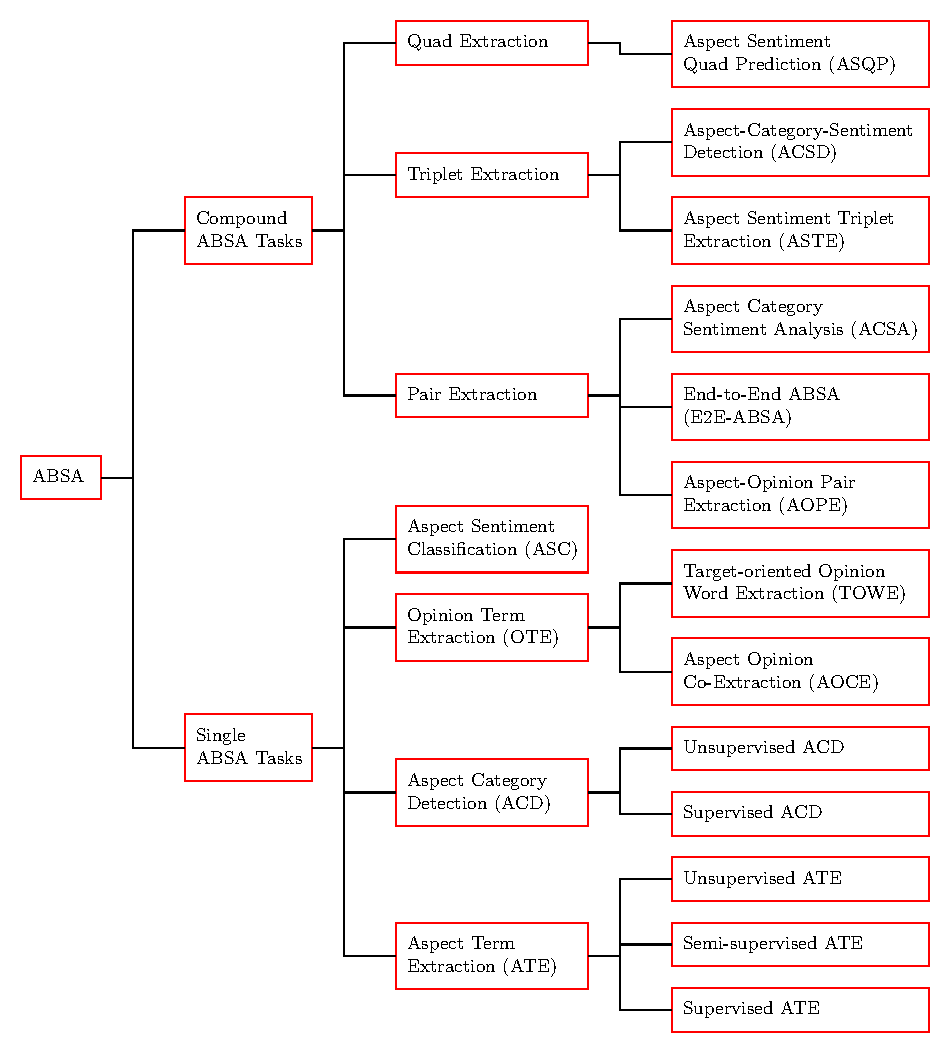
\includegraphics[width=\textwidth]{figures/absa_tasks.pdf}
	\caption{Taxonomía de las tareas de ABSA. Reconstruido de \citet{zhang_survey_2023}.}
	\label{fig:absa_tasks}
\end{figure}

En la presente tesis se adopta el paradigma \textbf{ACD + ASC}: la categoría de aspecto se predice mediante clasificación zero-shot vía NLI (Sección~\ref{subsec:zero_shot}) y, condicionalmente al aspecto detectado, se aplica un clasificador de sentimiento basado en un codificador Transformer con ajuste fino sobre reseñas en español (Sección~\ref{subsec:sentiment_models}). Esta elección está motivada por dos consideraciones: (i) la ausencia de datos etiquetados a nivel de aspecto para Pueblos Mágicos hace inviables los enfoques supervisados, y (ii) el conjunto de aspectos relevantes varía entre tipos de establecimiento, lo cual se acomoda naturalmente a un esquema condicional en el que el conjunto de etiquetas candidatas se ajusta dinámicamente sin reentrenar.

% -------------------------------------------------------------------------

\subsection{Detección de fronteras de oración} \label{subsec:sbd}

Antes de aplicar cualquier modelo de clasificación a las reseñas, el texto debe segmentarse en unidades coherentes sobre las que se predicen los aspectos. Esta tarea, conocida como \textit{Sentence Boundary Detection} (SBD) o \textit{Sentence Boundary Disambiguation}, consiste en identificar el conjunto de posiciones del texto que corresponden a finales de oración. Aunque suele tratarse como un paso de preprocesamiento trivial, los errores en SBD se propagan a las etapas posteriores de la cadena de NLP, degradando el rendimiento de etiquetadores morfosintácticos, analizadores semánticos y clasificadores \citep{read_sentence_2012}. Para el caso del ABSA, una segmentación deficiente puede unir en un mismo fragmento juicios de polaridad opuesta sobre aspectos distintos, frustrando el principio de granularidad fina sobre el que se sustenta la tarea.

La dificultad principal del SBD reside en la \emph{ambigüedad del punto}: el grafema \texttt{`.'} actúa simultáneamente como marcador de final de oración, parte de abreviaturas (e.g., \textit{Sr.}, \textit{Av.}), separador de números ordinales o decimales e indicador de iniciales. Las aproximaciones a esta tarea se agrupan en tres familias: (i) sistemas \textit{basados en reglas}, que combinan heurísticas con listas curadas de abreviaturas; (ii) sistemas \textit{supervisados}, entrenados sobre corpus con fronteras anotadas mediante clasificadores de máxima entropía, SVM o redes neuronales; y (iii) sistemas \textit{no supervisados}, que infieren las fronteras a partir de regularidades distribucionales del propio corpus, sin requerir anotación manual. La revisión empírica de \citet{read_sentence_2012} sobre nueve sistemas y cuatro corpus muestra una variabilidad de rendimiento considerable entre dominios y tipos de texto, y advierte que las evaluaciones tradicionales sobre prosa formal (Wall Street Journal, Brown) sobrestiman la robustez de los segmentadores cuando se aplican a contenido generado por usuarios, donde la puntuación es irregular y el registro es informal.

En este trabajo se adopta el segmentador no supervisado \textbf{Punkt} \citep{kiss_unsupervised_2006}. La hipótesis central de Punkt es que la mayor parte de las ambigüedades del punto puede resolverse identificando primero las abreviaturas presentes en el corpus, ya que toda posición que no siga a una abreviatura se clasifica directamente como frontera. Una abreviatura se caracteriza, sin información contextual, mediante tres propiedades del tipo léxico:
\begin{itemize}
	\item \textbf{Colocación con el punto.} La palabra truncada y el punto final forman una colocación estricta; se cuantifica con la verosimilitud logarítmica
	      \begin{equation} \label{eq:punkt_llr}
		      \log\lambda(w, \texttt{`.'}) = -2 \log \frac{L(p_0; k_1, n_1)\, L(p_0; k_2, n_2)}{L(p_1; k_1, n_1)\, L(p_2; k_2, n_2)}
	      \end{equation}
	      donde $L(\cdot)$ es la verosimilitud bajo el modelo binomial, $k_i, n_i$ son conteos de coocurrencia y $p_0, p_1, p_2$ son las estimaciones bajo independencia y dependencia, respectivamente.
	\item \textbf{Brevedad del tipo.} Las abreviaturas tienden a ser cortas; la probabilidad de que un tipo $w$ sea abreviatura decae con su longitud.
	\item \textbf{Puntos internos.} Los tipos que contienen puntos en su interior (e.g., \textit{a.m.}) son fuertes candidatos a abreviatura.
\end{itemize}
La combinación multiplicativa de estos tres factores produce un \textit{score} de abreviatura por tipo, sobre el que un umbral global decide la clasificación. Una segunda fase a nivel de \textit{token} resuelve los casos restantes (números ordinales, iniciales y palabras que pueden ser tanto abreviaturas como ordinarias) usando rasgos contextuales como la capitalización de la palabra siguiente. \citet{kiss_unsupervised_2006} reportan una precisión media del $98.74\%$ sobre corpus periodísticos en once idiomas (incluyendo el español) sin ninguna adaptación específica al idioma, lo que justifica su elección como segmentador en este trabajo, dado el carácter multilingüe-agnóstico de su entrenamiento y la ausencia de un corpus de reseñas turísticas en español con fronteras de oración anotadas. La salida de Punkt define los fragmentos $\{t_1, \ldots, t_F\}$ sobre los que se aplican posteriormente la detección de aspecto y la clasificación de sentimiento.

% --------------------------------------------------------------
\subsection{Clasificación zero-shot vía NLI} \label{subsec:zero_shot}

La clasificación zero-shot tiene por objetivo asignar etiquetas a un texto sin disponer de ejemplos anotados para las clases objetivo \citep{yin_benchmarking_2019}. Formalmente, se considera el escenario \textit{label-fully-unseen}: aprender un clasificador $f : \mathcal{X} \to \mathcal{Y}$ tal que $f$ no observa ningún dato etiquetado específico para las clases en $\mathcal{Y}$ durante su entrenamiento. Esta formulación es particularmente adecuada para ACD en dominios sin \textit{benchmarks} curados, ya que permite definir el conjunto de aspectos $\mathcal{C}$ post-hoc y modificarlo sin reentrenamiento.

\citet{yin_benchmarking_2019} proponen tratar la clasificación zero-shot como un problema de \textit{Natural Language Inference} (NLI). La tarea de NLI es una tarea de clasificación supervisada que consiste en determinar la relación entre una premisa $t$ y una hipótesis $h$ mediante tres clases: implicación, contradicción y neutralidad \citep{maccartney2009natural}. La idea consiste en convertir cada etiqueta candidata $c \in \mathcal{C}$ en una hipótesis $h_c$ mediante una plantilla parametrizada (e.g., ``\textit{Este texto habla sobre $\{c\}$.}'') y, dada una premisa $t$ (la oración o reseña), evaluar la probabilidad de implicación usando un modelo NLI preentrenado. La etiqueta predicha es entonces:
\begin{equation} \label{eq:zeroshot_nli}
	\hat{c} = \arg\max_{c \in \mathcal{C}} \Pr\!\left(\text{entailment} \mid t, h_c\right)
\end{equation}
En el caso multi-etiqueta, se aplica un umbral $\tau$ y se devuelven $\{c \in \mathcal{C} : \Pr(\text{entailment} \mid t, h_c) > \tau\}$. \citet{yin_benchmarking_2019} muestran que un modelo BERT ajustado finamente sobre MNLI \citep{williams_broad-coverage_2018} generaliza competitivamente a tareas de detección de aspectos no vistas, superando enfoques basados en \textit{embeddings} estáticos (Word2Vec, ESA) por márgenes significativos en clases no vistas.

% --------------------------------------------------------------
\subsection{Transformers para clasificación de sentimiento} \label{subsec:sentiment_models}

La subtarea ASC se formula como un problema de clasificación supervisada sobre representaciones contextuales producidas por un codificador Transformer. Dada una secuencia de entrada $t = (w_1, \ldots, w_n)$, los modelos tipo BERT/RoBERTa anteponen un token especial $\texttt{[CLS]}$ y producen, tras $L$ capas de \textit{self-attention}, una matriz de \textit{embeddings} contextuales $\mathbf{H} \in \mathbb{R}^{(n+1) \times d}$. Para tareas de clasificación a nivel de oración se adopta el vector $\mathbf{h}_{\texttt{[CLS]}} \in \mathbb{R}^d$ asociado al token especial como representación agregada de la secuencia, y se añade una cabeza de clasificación lineal:
\begin{equation} \label{eq:cls_head}
	\Pr(s \mid t) = \mathrm{softmax}\!\left(\mathbf{W}\, \mathbf{h}_{\texttt{[CLS]}} + \mathbf{b}\right), \qquad \mathbf{W} \in \mathbb{R}^{|\mathcal{S}| \times d},\ \mathbf{b} \in \mathbb{R}^{|\mathcal{S}|}
\end{equation}
donde $\mathcal{S}$ es el conjunto de clases. Los parámetros de la cabeza, junto con los del codificador, se ajustan minimizando la entropía cruzada sobre un corpus etiquetado de la tarea \textit{downstream}. Este esquema transfiere el conocimiento lingüístico capturado durante el preentrenamiento a tareas con relativamente pocos ejemplos etiquetados, superando consistentemente a las arquitecturas recurrentes y a los enfoques léxicos en clasificación de sentimiento \citep{do_deep_2019}.

Para el español existen varios modelos base ampliamente utilizados --- BETO \citep{CaneteCFP2020}, RoBERTuito \citep{perez-etal-2022-robertuito} --- que difieren en el corpus de preentrenamiento y, consecuentemente, en el dominio en el que mejor generalizan \citep{do_deep_2019}. El modelo seleccionado en este trabajo\footnote{\url{https://huggingface.co/vg055/roberta-base-bne-finetuned-TripAdvisorDomainAdaptation-finetuned-e2-RestMex2023-polaridadDA-V1}} parte de un RoBERTa base \citep{DBLP:journals/corr/abs-1911-02116} preentrenado sobre la Biblioteca Nacional de España (BNE) y posteriormente adaptado al dominio TripAdvisor mediante \textit{fine-tuning} para clasificación de sentimiento de granularidad fina, produciendo cinco clases ordinales:
\begin{equation*}
	\mathcal{S} = \{\text{Muy Negativo}, \text{Negativo}, \text{Neutral}, \text{Positivo}, \text{Muy Positivo}\}
\end{equation*}
La granularidad de cinco clases preserva información entre diferentes niveles de satisfacción y resulta consistente con la escala de 1 a 5 estrellas que usualmente se asigna en el dominio turístico.

%% ============================================================
%% 2.4  SISTEMAS DE RECOMENDACIÓN CON ABSA
%% ============================================================
\section{Sistemas de recomendación con ABSA} \label{sec:absa_rs}

El análisis de sentimientos basado en aspectos produce, para cada reseña asociada a un par usuario-ítem, un conjunto de pares aspecto-sentimiento que indica qué atributos del ítem menciona el usuario y con qué polaridad los valora. Esta información de granularidad fina permite enriquecer a los sistemas de recomendación clásicos, que por sí solos disponen únicamente de una calificación numérica global por interacción y descartan los matices expresados en el texto. El modelo de referencia para incorporar dichas señales es el \textit{Explicit Factor Model} (EFM) propuesto por \citet{zhang_explicit_2014}, cuyas representaciones aspectuales constituyen la base de la propuesta desarrollada en esta tesis.

El EFM organiza la información extraída por ABSA en dos matrices que describen, respectivamente, las preferencias de los usuarios y las cualidades de los ítems sobre un espacio común de aspectos. Se denota por $\mathcal{U}$ al conjunto de usuarios, por $\mathcal{I}$ al de ítems y por $\mathcal{A}$ al de aspectos considerados.

La \textit{matriz de atención del usuario} $\mathbf{X} \in \mathbb{R}^{|\mathcal{U}| \times |\mathcal{A}|}$ codifica la importancia que cada usuario $u$ concede al aspecto $a$. Su valor crece con la frecuencia con que el usuario menciona ese aspecto en sus reseñas, frecuencia que se transforma mediante una sigmoide para acotar el resultado en el intervalo $[1, N]$, donde $N$ es el extremo superior de la escala de calificación:
\begin{equation} \label{eq:efm_X}
	X_{u,a} = 1 + (N - 1) \left(\frac{2}{1 + \exp(-t_{u,a})} - 1\right),
\end{equation}
con $t_{u,a}$ el número de menciones del aspecto $a$ por parte del usuario $u$. La intuición subyacente es que un aspecto mencionado con insistencia revela una preocupación genuina del usuario por ese atributo.

La \textit{matriz de calidad del ítem} $\mathbf{Y} \in \mathbb{R}^{|\mathcal{I}| \times |\mathcal{A}|}$ codifica qué tan bien evaluado está cada ítem $i$ en el aspecto $a$. Para ello combina el sentimiento promedio $s_{i,a}$ que la comunidad expresa sobre ese aspecto con el volumen de menciones $t_{i,a}$ que lo respaldan, de modo que una valoración positiva sostenida por muchas opiniones pesa más que un juicio aislado:
\begin{equation} \label{eq:efm_Y}
	Y_{i,a} = 1 + \frac{N - 1}{1 + \exp(-t_{i,a} \cdot s_{i,a})}.
\end{equation}

Con ambas matrices, el EFM predice la calificación que el usuario $u$ otorgaría al ítem $i$ sumando dos contribuciones. La primera es un término explícito, el producto interno entre la atención del usuario y la calidad del ítem en el espacio de aspectos, que resulta directamente interpretable. La segunda es un término latente al estilo de la factorización matricial, que captura patrones residuales no explicados por los aspectos:
\begin{equation} \label{eq:efm_pred}
	\hat{r}_{u,i} = \alpha \, \frac{\mathbf{X}_u^\top \mathbf{Y}_i}{|\mathcal{A}|} + (1 - \alpha) \, \mathbf{p}_u^\top \mathbf{q}_i,
\end{equation}
donde $\mathbf{p}_u$ y $\mathbf{q}_i$ son los vectores latentes de usuario e ítem, y el escalar $\alpha \in [0, 1]$ regula el peso relativo de cada contribución. La virtud del término explícito es que vincula la salida del recomendador con la representación aspectual extraída del texto. En el modelo original esto habilita justificaciones legibles de la recomendación, como afirmar que se sugiere Taxco porque el usuario valora la \texttt{cultura} y la \texttt{naturaleza}, dos aspectos que la comunidad evalúa de forma sobresaliente en ese pueblo.

Conviene precisar el alcance con el que esta tesis adopta el EFM. De este modelo se reutilizan las dos matrices de aspectos, la de atención del usuario $\mathbf{X}$ y la de calidad del ítem $\mathbf{Y}$, por su carácter interpretable y porque reflejan de forma transparente las preferencias y las cualidades en términos de aspectos. No se instancia, en cambio, el modelo completo: la propuesta prescinde del término de factores latentes $\mathbf{p}_u^\top \mathbf{q}_i$ de la Ecuación~(\ref{eq:efm_pred}). El componente basado en contenido del híbrido emplea solamente una versión normalizada del término explícito,
\begin{equation} \label{eq:cbquality}
	\hat{r}_{u,p} = \frac{\sum_{a \in \mathcal{A}} X_{u,a}\, Y_{p,a}}{\sum_{a \in \mathcal{A}} X_{u,a}},
\end{equation}
de manera que la predicción se interpreta como el grado de correspondencia entre la importancia que el usuario asigna a cada aspecto y la calidad del pueblo en ese mismo aspecto, sin recurrir a ninguna factorización latente. La construcción concreta de $\mathbf{X}$ e $\mathbf{Y}$ a partir del corpus REST-MEX y su combinación con el componente colaborativo en el recomendador híbrido se desarrollan en el capítulo de metodología.
